\chapter{Test und Evaluation}

Bisher wurde der Feasibility Check nur wenig von tatsächlichen Endanwendern genutzt; sämtliche bisher durchgeführten Tests beziehen sich ausschließlich auf Unittests der Backend-Logik. Diese Unittests wurden mit großem Aufwand und hoher Sorgfalt entwickelt, um sicherzustellen, dass die bestehende Logik auch in Zukunft stabil bleibt und Änderungen keine unerwarteten Fehler verursachen.

\section{Unittests}

Die Entwicklung der Unittests für den Feasibility Check gestaltete sich als besonders anspruchsvoll. Dies liegt vor allem daran, dass es nicht ausreicht, der Methode \texttt{FeasibilityCheck()} einfache fehlerhafte Eingaben zu übermitteln. Vielmehr erwartet diese Methode eine existierende Test-ID, die in der Datenbank vorhanden ist und im Regelfall mit Operationen sowie zugehörigen Parametern befüllt sein muss. Zusätzlich hängt das Ergebnis des Feasibility Checks von mehreren Faktoren ab, wie etwa der Feasibility-Konfiguration, den einzelnen Condition- und Equipment-Checks, der \texttt{op\_data\_param\_type}-Tabelle sowie den in der Datenbank hinterlegten Maschinen.

Aufgrund dieser Komplexität ist es notwendig, gezielt ''Fake-Daten'' in einer Testdatenbank anzulegen. Aufbauend auf diesen Testdaten wird der Feasibility Check ausgeführt und das Ergebnis hinsichtlich Korrektheit und Vollständigkeit validiert. Nach erfolgreicher Überprüfung erfolgt eine sichere Entfernung der ''Fake-Daten'', um die Integrität der Datenbank zu gewährleisten.

Um diesen Prozess zu vereinfachen, wurde die Klasse \texttt{FeasibilityCheckScenario} eingeführt, die auf einer Projektszenario-Klasse basiert. Dieses Konzept stellt eine Sammlung einfacher Methoden bereit, mit denen entweder ein standardisierter Feasibility-Test oder ein spezifischer Test mit vorgegebenen Inhalten angelegt werden kann. Über public Boolean-Parameter in der \texttt{FeasibilityCheckScenario}-Klasse können verschiedene Szenarien aktiviert werden, die intern zur Erzeugung der entsprechenden Fake-Daten führen. Beispielsweise kann das Szenario \texttt{PlanValueOutOfRange} aktiviert werden, um einen Testfall zu simulieren, bei dem der PlanValue außerhalb des erlaubten Bereichs liegt. Ein weiteres Beispiel ist das Szenario \texttt{WrongMachineDate}, bei dem eine Maschine, die normalerweise für den Test zugelassen wäre, mit einem inkorrekten Datum erstellt wird. Standardmäßig sind alle Szenarien deaktiviert und können je nach Bedarf einzeln oder in Kombination aktiviert werden. Abbildung~\ref{fig:unittests-parameters} veranschaulicht die möglichen Boolean-Parameter, die als Szenarien innerhalb der \texttt{FeasibilityCheckScenario}-Klasse dienen.

\begin{figure}[!htb]
    \centering
    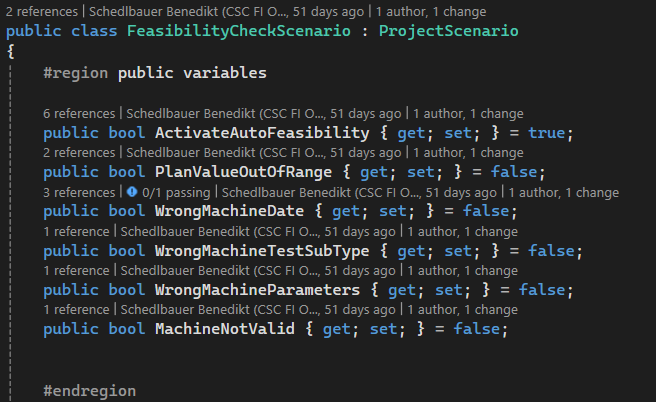
\includegraphics[width=1\textwidth]{bilder/unittests-parameters.png}
    \caption{Boolean-Parameter der \texttt{FeasibilityCheckScenario}-Klasse}
    \label{fig:unittests-parameters}
\end{figure}

Durch diese abstrahierte Vorgehensweise lassen sich die umfangreichen Unittests strukturiert und effizient umsetzen. Zwei Beispiel-Unittests sind in Abbildung~\ref{fig:unittestcases} dargestellt. Hierbei legt die Methode \texttt{CreateDefaultFeasibilityProject()} einen Default-Test an, der jeweils mit einer Operation und einem Parameter befüllt ist, um das Testszenario zu vereinfachen. Anschließend generiert die Methode \texttt{CreateMockData()} in der Datenbank alle erforderlichen ''Fake-Daten'' bzw. passt bestehende Datensätze an, beispielsweise in der Feasibility-Konfigurationstabelle. Die Erstellung dieser ''Fake-Daten'' erfolgt abhängig von den eingestellten Boolean-Parametern, sodass die entsprechenden Szenarien erfüllt werden. Im zweiten Unittest, wie in Abbildung~\ref{fig:unittestcases} gezeigt, wurde beispielsweise das Szenario \texttt{WrongMachineDate} aktiviert. Danach wird über die Methode \texttt{PerformFeasibilityCheck()} der Feasibility Check ausgeführt, wobei das zurückgelieferte Ergebnis abschließend evaluiert wird. Ein automatisierter Cleanup-Mechanismus sorgt schließlich dafür, dass die initial angelegten Fake-Daten sicher wieder aus der Datenbank entfernt werden.

\begin{figure}[!htb]
    \centering
    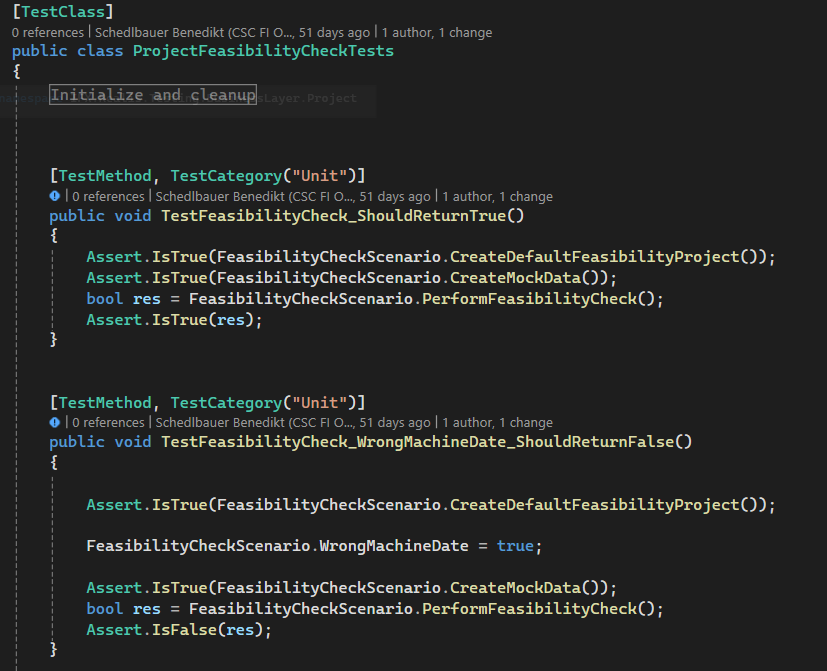
\includegraphics[width=1\textwidth]{bilder/unittestcases.png}
    \caption{Unittests für den Feasibility Check}
    \label{fig:unittestcases}
\end{figure}

Die Unittests sind in ein automatisiertes Test-Framework integriert, sodass bei jeder Änderung der Backend-Logik automatisch überprüft wird, ob alle Testfälle weiterhin erfolgreich durchlaufen werden. Diese Vorgehensweise unterstützt die kontinuierliche Qualitätssicherung und trägt maßgeblich zur Stabilität und Wartbarkeit des Systems bei.

\section{Ergebnisse der Tests}
Darstellung der Testergebnisse und ihrer Bedeutung.

\section{Evaluation des Systems}
Bewertung der Lösung hinsichtlich der definierten Anforderungen.

Die implementierten Unittests bilden somit eine solide Grundlage für die Qualitätssicherung des Feasibility Checks. Dennoch bleibt die Integration des gesamten Systems unter realen Betriebsbedingungen ein zukünftiges Ziel. In diesem Zusammenhang sind weitere Testmethoden wie Integrationstests und Usability-Tests vorgesehen, um sowohl die technische Robustheit als auch die Anwenderfreundlichkeit des Systems umfassend zu evaluieren.